%% LyX 2.3.4.4 created this file.  For more info, see http://www.lyx.org/.
%% Do not edit unless you really know what you are doing.
\documentclass[british]{article}
\usepackage[T1]{fontenc}
\usepackage[utf8]{inputenc}
\usepackage{babel}
\usepackage{graphicx}
\usepackage[unicode=true,pdfusetitle,
 bookmarks=true,bookmarksnumbered=false,bookmarksopen=false,
 breaklinks=false,pdfborder={0 0 1},backref=false,colorlinks=false]
 {hyperref}

\makeatletter

%%%%%%%%%%%%%%%%%%%%%%%%%%%%%% LyX specific LaTeX commands.
%% Because html converters don't know tabularnewline
\providecommand{\tabularnewline}{\\}

\makeatother

\begin{document}
\title{Predicting Tennis Outcomes Using Random Walks}
\author{Tomáš Kouřim}
\date{}
\maketitle
\begin{abstract}
Recently introduced random walk model showed its possible use in predicting
tennis men Grand Slam tournaments outcomes. The model was then further
examined and its theoretical background was described in more detail.
In this paper the model is trained using the most recent data and
then applied for in-play betting against a bookmaker. Different betting
strategies are tested and the overall performance of the model is
evaluated.
\end{abstract}

\section{Introduction}

Random walk was first introduced by K. Pearson over 100 years ago
\cite{pearson1905problem}. Since then the concept was further elaborated,
the random walk was described in much detail and many alternatives
of the original model were introduced. One of the most recent variations
of a random walk is a random walk with varying probabilities, a concept
introduced recently by the authors \cite{ja2017ddny}. It is based
on a similar concept of a random walk with varying step size introduced
by L. Turban \cite{turban2010random}. This model seems particularly
well suited to model different sporting events, especially tennis
matches.

A proper model of a tennis match, and more generally any sporting
event, is of a great value. It can serve the athletes and their coaches
to improve their strengths and eliminate weaknesses, it can bring
new insides into the game and it is especially useful in the sports
betting industry. Such model can be used by bookmakers to provide
more accurate odds, it can used by professional bettors to gain an
edge against the bookmakers and a robust model can also help to detect
fraudsters selling their matches or betting on games where the result
was agreed long before the game even started.

The paper is organized as follows. Next chapter briefly introduces
the model used for tennis modeling. Section \ref{sec:Data-description}
provides general description of the data used, Section \ref{sec:Optimal-model-selection}
describes the model fitting procedure. In Chapter \ref{sec:Model-application-for}
the model is tested against a database of real life bookmaker's odds
and its performance is evaluated. Section \ref{sec:Conclusion} concludes
this paper.

\section{Random walk with varying probability\label{sec:Random-walk-with}}

The idea behind the model of a random walk with varying probability
is that the probability distribution of the next step depends directly
on the result of the previous step in the following manner. Let us
have a basic random walk with steps $X\in\{-1,\,1\}$ with Bernoulli
distribution depending on a parameter $p$ so that $P(x=1)=p$ and
$P(x=-1)=1-p$. After each step this probability is altered using
a memory coefficient $\lambda$ and the result of previous step. We
can define two major types of random walk with varying probability -\emph{
success punishing} and\emph{ success rewarding}. The first denotes
that every time an event occurs, the probability of its repetition
decreases, i.e. if step $X_{t}=1$ then the probability the next step
 $X_{t+1}=1$ decreases by a parameter $\lambda$ so that $p_{t+1}=\lambda p_{t}$.
For the\emph{ success rewarding} model, the opposite holds and every
time an event occurs, the probability of its repetition increases.

The model can be further refined by using two separate parameters,
one for each direction, i.e. $\lambda=[\lambda_{1},\,\lambda_{2}]$.
Again, there can be\emph{ success punishing} and\emph{ success rewarding}
model. Thus, together there are four basic model variants. Formal
definitions of all four model variants and their detailed description
together with the derivation of useful formulas can be found in \cite{ja2019apmat}.

\subsection{Application for tennis modeling}

The random walk model can be applied to model any discrete time random
process. Such processes often occur in sports, especially in sports
played not for certain amount of time, but for certain amount of points.
These sports include for example volleyball, badminton or tennis.
Tennis seems as particularly interesting sport in terms of discrete
random processes. There are several such processes. Series of matches
can be considered a discrete random process, the sets played within
a match, games within a set, points within a game or even strokes
within a point, they all can be considered discrete random processes.
In this paper, the model of a random walk with varying probability
was used to model the sets played within a match.

\section{Data description\label{sec:Data-description}}

For the purpose of this paper an automatic data gathering tool was
created. This tool was continuously scraping data from\emph{ www.tipsport.cz},
the website of the biggest Czech bookmaker, gathering provided odds
for the winner of the first set of each match and, if available, also
the\emph{ in-play} odds for each set played. The tool also stored
the results of each particular set played. The tool was developed
using the Python programming language with the help of Selenium framework.
PostgreSQL database deployed on Digital Ocean infrastructure was used
for data storage. For the purpose of this paper, data from February
until May 2021 was available.

The data was split into training and testing datasets. Training dataset
contains odds and results of matches played from February till the
end of April, May matches represent the testing dataset. In the training
dataset, there were 12 372 matches. Complete information, i.e. both
odds and result, were available for 3 365 matches (mostly because
the bookmaker did not provide\emph{ in-play} odds for the matches).
As the matches are played as\emph{ best-of-three} (or\emph{ best-of-five}
in case of 2021 ATP Australian Open) there were 8 310 sets played
where all information required for the presented model was available.
The testing dataset contains 3 076 matches, 1 150 of which with complete
information, and there are 2 796 relevant sets.

\section{Model training\label{sec:Optimal-model-selection}}

As mentioned in Section \ref{sec:Random-walk-with}, there are four basic
variants of the model altogether with two (or three in case of $\lambda=[\lambda_{1},\,\lambda_{2}]$)
unknown parameters. Model training thus consists of two steps, best
model variant selection and finding the optimal parameter.

\subsection{Starting probability selection\label{subsec:Starting-probability-selection}}

The first unknown parameter of the model is the starting probability
$p_{0}$. In tennis modeling, coefficient $p_{0}=p_{A}$ means the
probability that Player A will win the first set. This probability
(or its estimate) is implicitly given by the odds $o=[o_{A},\,o_{B}]$
provided by bookmaker. Roughly, $p_{A}\widetilde{=}\frac{1}{o_{A}}$.
This estimate can be further refined. First, for typical odds there
holds that $\frac{1}{o_{A}}+\frac{1}{o_{B}}>1$ (i.e., typically the
bookmaker provides\emph{ subfair} odds with bookmaker's winning margin).
First step is thus the normalization of odds. It turns out that the
simple normalization, i.e. $p_{A}=n_{1}(o)=\frac{\frac{1}{o_{A}}}{\frac{1}{o_{A}}+\frac{1}{o_{B}}}$
does not provide reasonable results. In fact, bookmaker's margin is
usually unevenly distributed towards the outsider. Therefore, an alternative
normalization function can be used
\begin{equation}
p_{A}=n_{2}(o)=\frac{1}{o_{A}}+\frac{o_{A}o_{B}-o_{A}-o_{B}}{o_{B}(o_{A}+o_{B})}.\label{eq:n2_normalization}
\end{equation}
This can be further improved by introducing a third normalization
function $\mu(o,t)$, with a real parameter $t$ linearly extrapolating
$n_{1}$ and $n_{2}$ such that $\mu(o,0)=n_{2}(o)$ and $\mu(o,2)=n_{1}(o)$ \cite{ja2015ddny}.

To obtain reasonable estimation of the model parameter $p_{0}$ from
provided odds, the first step is to estimate the parameter $t$. This
was done using the maximal likelihood estimate method and the training
set. Bookmaker's odds for the first set and the actual result of the
first set were used. The likelihood function is defined as
\[
L=\prod_{i=1}^{N}(x_{i}\mu(o_{i},\,t)+(1-x_{i})(1-\mu(o_{i},\,t)),
\]
where $N$ is the number of matches in the training dataset, $o_{i}$
is the bookmaker's odds for the first set in the $i-th$ match and
$x_{i}$ is the result of the first set in the $i-th$ match, $x_{i}=1$
if Player A won the set, $x_{i}=0$ otherwise. For computational reasons
the\emph{ log-likelihood} $L_{l}=ln(L)$ was used, i.e. the function
\[
L_{l}=\sum_{i=1}^{N}ln(x_{i}\mu(o_{i},\,t)+(1-x_{i})(1-\mu(o_{i},\,t)).
\]
Numerical methods, namely the function\emph{ minimize\_scalar} from
the Python SciPy package, were used to obtain optimal value of parameter
$t=4.03e-06$. We can thus consider $t=0$ and use function $n_{2}$
for normalization.

\subsection{Model and memory parameter selection\label{subsec:Model-selection}}

For each match with data for at least 2 sets available (i.e. with
at least 1 prediction opportunity), the first set winning probability
$p_{0}$ was derived using the procedure and parameter from previous
paragraph. Then, for each of the four model variants the optimal value
of coefficient $\lambda$ was found again using the training dataset and the maximum log-likelihood
estimate
\[
L_{l}=\sum_{i=1}^{N}\sum_{j=1}^{N_{i}}ln(x_{ij}p_{ij}+(1-x_{ij})(1-p_{ij})),
\]
where $N$ denotes the number of matches in testing dataset, $N_{i}$
the number of predictable sets in $i-th$ match, $x_{ij}$ is the
result of the $j-th$ set in the $i-th$ match, $x_{ij}=1$ if Player
A won the set, $x_{ij}=0$ otherwise and $p_{ij}$ is the probability of Player
A winning the set computed using the currently considered model variant.

Finally, the Akaike Information Criterion $AIC=2k-2L_{l}$, which
considers the number of parameters to find the optimal model, was
used. Here $k$ is the number of model parameters and $L_{l}$ is the
maximal log-likelihood.

Based on the available training data the\emph{ single lambda success
rewarding} model variant was selected, with $\lambda=0.826$ and $p_{0}$
computed for each match using the $n_{2}$ normalization function
defined in (\ref{eq:n2_normalization}).

\section{Model application for in-play betting\label{sec:Model-application-for}}




To test the quality of the model, following experiment was performed.
For each match in the testing dataset, first the starting probability was
derived using the procedure described in Section \ref{subsec:Starting-probability-selection}.
Then for each set played, the
set winning probability was computed using the\emph{ success rewarding}
model and memory parameter $\lambda=0.826$ as specified in Section
\ref{subsec:Model-selection}. Finally, this probability was compared to odds
provided by the bookmaker and a virtual bet was made.

\begin{table}
\begin{centering}
\begin{tabular}{|c|c|c|c|c|c|}
\hline 
Strategy & Bet & $E(w)$ & $E(w|p=\frac{1}{o})$ & $Var(w)$ & $Var(w|p=\frac{1}{o})$\tabularnewline
\hline 
\hline 
Naive & $1$ & $po-1$ & $0$ & $po^{2}(1-p)$ & $o(1-\frac{1}{o}$)\tabularnewline
\hline 
Odds & $\frac{1}{o}$ & $p-\frac{1}{o}$ & $0$ & $p(1-p)$ & $\frac{1-\frac{1}{o}}{o}$\tabularnewline
\hline 
Prob. & $p$ & $p(po-1)$ & $0$ & $p^{3}o^{2}(1-p)$ & $\frac{1-\frac{1}{o}}{o}$\tabularnewline
\hline 
General & $u$ & $u(po-1)$ & $0$ & $u^{2}po^{2}(1-p)$ & $u^{2}o(1-\frac{1}{o})$\tabularnewline
\hline 
\end{tabular}
\par\end{centering}
\caption{\label{tab:strategies}Theoretical values of wins and variances for
different betting strategies. $p$ is the probability of winning,
$o$ is the odds provided by bookmaker.}
\end{table}

Choosing the correct betting strategy is one of the key elements of
successful betting. It depends on the underlying model, available
bookmaker's odds, bankroll, internal bookmaker's policies and many
other parameters. There exists a large number of possible approaches
and the detailed description of them is beyond the scope of this paper.
For testing purposes, there were three basic strategies tested. First,
the naive betting strategy, where simply $1$ unit was bet every time.
Then, the probability based strategy, where $p$ (probability of winning)
units was bet. Finally the odds based strategy, where $\frac{1}{odds}$ units 
was bet. The strategies differ in the expected wins and their variance.
The theoretical properties of the betting strategies can be observed
in Table \ref{tab:strategies} with the special case where $p=\frac{1}{a}$,
i.e. in case of \emph{fair} odds \cite{ja2015ddny}. Besides the different
betting amount strategies, it is also important to choose when to
bet. The basic strategy is to bet always when $p>\frac{1}{odds}$.
It turns out that it is more favorable to bet only when there is a
margin present, i.e. when $p>\frac{1}{odds}\cdot m$, where $m$ is
some margin parameter, $m\geq1.$

For $m=1.2$, i.e. $20\%$ margin, there are 65 virtual bets made
and a significant profit is achieved. One of the parameters to evaluate
a quality of a betting strategy is the return of investment (ROI),
i.e. $\frac{profit}{bankroll\,needed}.$ The naive betting yields $ROI=148\%$, probability based betting $ROI=98\%$
and odds based betting $ROI=111\%$. The development of the portfolio
balance can be seen in Figure \ref{fig:A-graph-showing}.

\begin{figure}
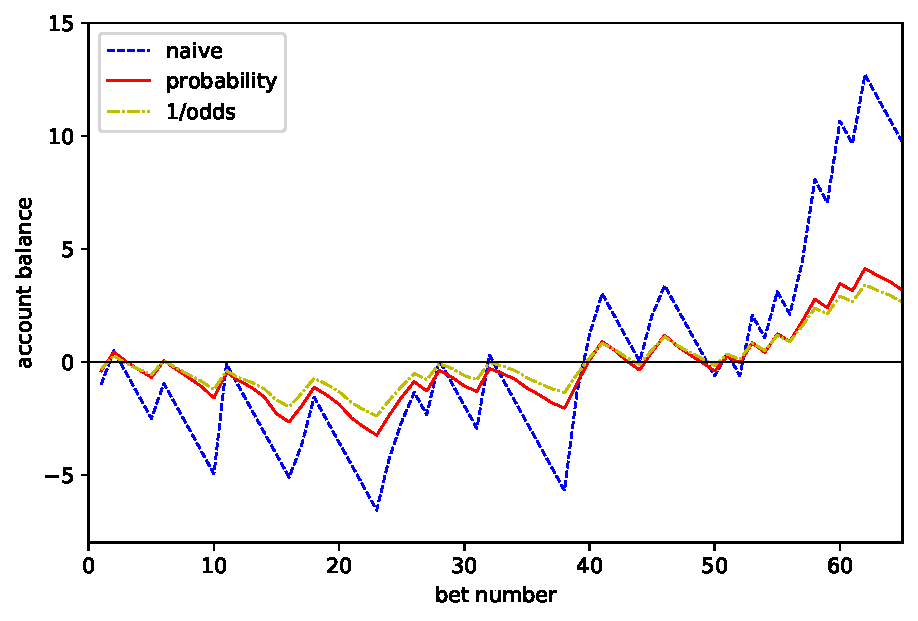
\includegraphics[width=0.9\textwidth]{account_balance_development}\caption{\label{fig:A-graph-showing}A graph showing the account balance development
for different betting strategies.}
\end{figure}





\section{Conclusion and future work\label{sec:Conclusion}}

In this paper, a recently introduced model of a random walk with varying
pro\-ba\-bilities was used to predict the development of a tennis match.
The quality of the predictions was tested against a real life odds
provided by a bookmaker and the results confirm big potential of the
model for tennis modeling. To better validate the model quality a
larger dataset has to be acquired. The model can be further improved,
for example by introducing a variable memory coefficient $\lambda$
or by combining the model with some of the more classical, regression
based approaches. This will be subject of a further research.

\section{Remarks\label{sec:Remarks}}

The source code containing all functionality mentioned in this article
is freely available as open source at GitHub\footnote{https://github.com/tomaskourim/mathsport2021}.
More results can be also obtained from the same repository. The data
used in this paper are available from the author upon request.

\bibliographystyle{plain}
\bibliography{doktknih}

\end{document}
